\documentclass[tikz]{standalone}
\usetikzlibrary{calc,positioning,shapes.multipart,shapes.misc,chains,arrows}

\begin{document}

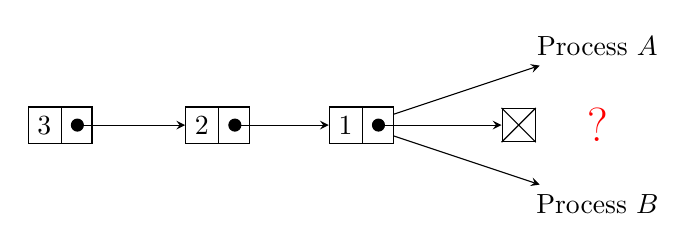
\begin{tikzpicture}[list/.style={rectangle split, rectangle split parts=2,
  draw, rectangle split horizontal}, >=stealth, start chain, distance=5mm and 5mm]

  \node[list,on chain] (A) {3};
  \node[list,on chain] (B) [right of=A] {2};
  \node[list,on chain] (C) {1};
  \node(P1) [above of=C,xshift=30mm] {Process $A$};
  \node(P2) [below of=C,xshift=30mm] {Process $B$};
  \node[on chain,draw,inner sep=6pt] (D) [right of=C] {};
  \node (dot) [right of=D,font=\LARGE\color{red}] {?}; 
  \draw (D.north east) -- (D.south west);
  \draw (D.north west) -- (D.south east);
  \draw[*->] let \p1 = (A.two), \p2 = (A.center) in (\x1,\y2) -- (B);
  \draw[*->] let \p1 = (B.two), \p2 = (B.center) in (\x1,\y2) -- (C);
  \draw[*->] let \p1 = (C.two), \p2 = (C.center) in (\x1,\y2) -- (D);
  \draw[<-] (P1) -- (C);
  \draw[<-] (P2) -- (C);

\end{tikzpicture}


\end{document}